% This file was created with tikzplotlib v0.10.1.
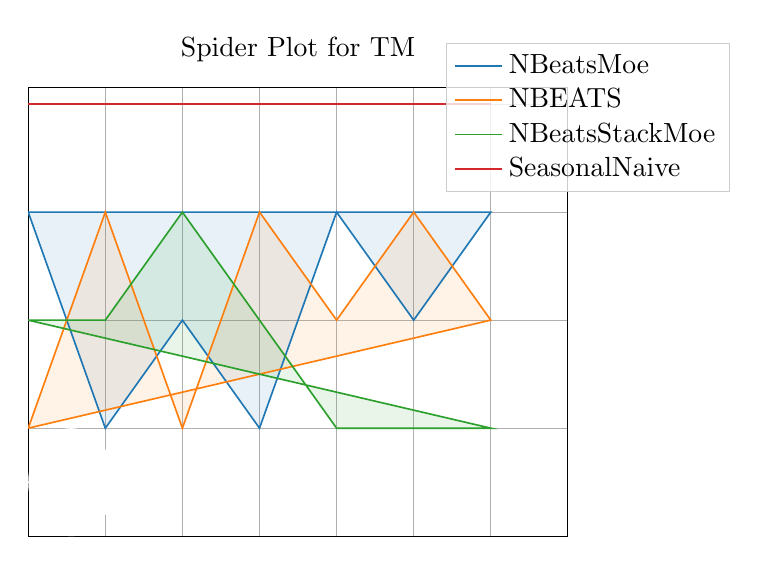
\begin{tikzpicture}

\definecolor{crimson2143940}{RGB}{214,39,40}
\definecolor{darkgray176}{RGB}{176,176,176}
\definecolor{darkorange25512714}{RGB}{255,127,14}
\definecolor{forestgreen4416044}{RGB}{44,160,44}
\definecolor{lightgray204}{RGB}{204,204,204}
\definecolor{steelblue31119180}{RGB}{31,119,180}

\begin{axis}[
legend cell align={left},
legend style={fill opacity=0.8, draw opacity=1, text opacity=1, at={(1.3,1.1)}, draw=lightgray204},
tick align=outside,
title={Spider Plot for TM},
x grid style={darkgray176},
xmajorgrids,
xmajorticks=false,
xmin=0, xmax=6.28318530717959,
xtick style={color=black},
xtick={0,0.897597901025655,1.79519580205131,2.69279370307697,3.59039160410262,4.48798950512828,5.38558740615393},
xticklabels={
  Overall,
  Exp. Shortfall,
  First horizon,
  Last horizon,
  On Hard,
  Anomalies,
  Non-anomalies
},
y grid style={darkgray176},
ymajorgrids,
ymajorticks=false,
ymin=0, ymax=4.15,
ytick style={color=black},
yticklabel style={anchor=west}
]
\path [draw=none, fill=steelblue31119180, fill opacity=0.1]
(axis cs:0,3)
--(axis cs:0.897597901025655,1)
--(axis cs:1.79519580205131,2)
--(axis cs:2.69279370307697,1)
--(axis cs:3.59039160410262,3)
--(axis cs:4.48798950512828,2)
--(axis cs:5.38558740615393,3)
--cycle;
\path [draw=none, fill=darkorange25512714, fill opacity=0.1]
(axis cs:0,1)
--(axis cs:0.897597901025655,3)
--(axis cs:1.79519580205131,1)
--(axis cs:2.69279370307697,3)
--(axis cs:3.59039160410262,2)
--(axis cs:4.48798950512828,3)
--(axis cs:5.38558740615393,2)
--cycle;
\path [draw=none, fill=forestgreen4416044, fill opacity=0.1]
(axis cs:0,2)
--(axis cs:0.897597901025655,2)
--(axis cs:1.79519580205131,3)
--(axis cs:2.69279370307697,2)
--(axis cs:3.59039160410262,1)
--(axis cs:4.48798950512828,1)
--(axis cs:5.38558740615393,1)
--cycle;
\path [draw=none, fill=crimson2143940, fill opacity=0.1]
(axis cs:0,4)
--(axis cs:0.897597901025655,4)
--(axis cs:1.79519580205131,4)
--(axis cs:2.69279370307697,4)
--(axis cs:3.59039160410262,4)
--(axis cs:4.48798950512828,4)
--(axis cs:5.38558740615393,4)
--cycle;
\path [draw=none, fill=white, line width=0pt]
(axis cs:1,0.5)
.. controls (axis cs:1,0.565659398403693) and (axis cs:0.987066530203795,0.630680341880369) .. (axis cs:0.961939766255643,0.691341716182545)
.. controls (axis cs:0.936813002307491,0.752003090484721) and (axis cs:0.899981596453154,0.807125184733393) .. (axis cs:0.853553390593274,0.853553390593274)
.. controls (axis cs:0.807125184733393,0.899981596453154) and (axis cs:0.752003090484721,0.936813002307491) .. (axis cs:0.691341716182545,0.961939766255643)
.. controls (axis cs:0.630680341880369,0.987066530203795) and (axis cs:0.565659398403693,1) .. (axis cs:0.5,1)
.. controls (axis cs:0.434340601596307,1) and (axis cs:0.369319658119631,0.987066530203795) .. (axis cs:0.308658283817455,0.961939766255643)
.. controls (axis cs:0.247996909515279,0.936813002307491) and (axis cs:0.192874815266607,0.899981596453154) .. (axis cs:0.146446609406726,0.853553390593274)
.. controls (axis cs:0.100018403546846,0.807125184733393) and (axis cs:0.0631869976925087,0.752003090484721) .. (axis cs:0.0380602337443566,0.691341716182545)
.. controls (axis cs:0.0129334697962046,0.630680341880369) and (axis cs:0,0.565659398403693) .. (axis cs:0,0.5)
.. controls (axis cs:0,0.434340601596307) and (axis cs:0.0129334697962045,0.369319658119631) .. (axis cs:0.0380602337443566,0.308658283817455)
.. controls (axis cs:0.0631869976925086,0.247996909515279) and (axis cs:0.100018403546846,0.192874815266607) .. (axis cs:0.146446609406726,0.146446609406726)
.. controls (axis cs:0.192874815266606,0.100018403546846) and (axis cs:0.247996909515279,0.0631869976925089) .. (axis cs:0.308658283817455,0.0380602337443567)
.. controls (axis cs:0.369319658119631,0.0129334697962046) and (axis cs:0.434340601596307,0) .. (axis cs:0.5,0)
.. controls (axis cs:0.565659398403693,0) and (axis cs:0.630680341880369,0.0129334697962046) .. (axis cs:0.691341716182545,0.0380602337443567)
.. controls (axis cs:0.752003090484721,0.0631869976925087) and (axis cs:0.807125184733393,0.100018403546846) .. (axis cs:0.853553390593274,0.146446609406726)
.. controls (axis cs:0.899981596453154,0.192874815266606) and (axis cs:0.936813002307491,0.247996909515279) .. (axis cs:0.961939766255643,0.308658283817455)
.. controls (axis cs:0.987066530203795,0.369319658119631) and (axis cs:1,0.434340601596307) .. (axis cs:1,0.5)
(axis cs:0.5,0.5)
(axis cs:1,0.5)
--cycle;
\addplot [semithick, steelblue31119180]
table {%
0 3
0.897597901025655 1
1.79519580205131 2
2.69279370307697 1
3.59039160410262 3
4.48798950512828 2
5.38558740615393 3
0 3
};
\addlegendentry{NBeatsMoe}
\addplot [semithick, darkorange25512714]
table {%
0 1
0.897597901025655 3
1.79519580205131 1
2.69279370307697 3
3.59039160410262 2
4.48798950512828 3
5.38558740615393 2
0 1
};
\addlegendentry{NBEATS}
\addplot [semithick, forestgreen4416044]
table {%
0 2
0.897597901025655 2
1.79519580205131 3
2.69279370307697 2
3.59039160410262 1
4.48798950512828 1
5.38558740615393 1
0 2
};
\addlegendentry{NBeatsStackMoe}
\addplot [semithick, crimson2143940]
table {%
0 4
0.897597901025655 4
1.79519580205131 4
2.69279370307697 4
3.59039160410262 4
4.48798950512828 4
5.38558740615393 4
0 4
};
\addlegendentry{SeasonalNaive}
\end{axis}

\end{tikzpicture}
